\chapter{Introducción}
\label{ch:intro}

Es un hecho que la \ac{ai} en general (y la \ac{ci} en particular) como área de conocimiento ha experimentado un creciente interés en los últimos años. Esto no siempre ha sido así, ya que después de un nacimiento muy esperanzador, con mucho optimismo, le siguieron unas épocas de apenas avance (ver cuadro~\ref{tbl:ai-timeline}). Sin embargo, en la actualidad es muy difícil encontrar un campo que no se beneficie directamente de sus técnicas.

\begin{margintable}
	\caption{Línea temporal de los principales hitos en la \glsentrytext{ai}. Actualmente la \glsentrytext{ai} está ofreciendo resultados muy prometedores áreas como la conducción autónoma, el procesamiento del lenguaje natural o el análisis de sentimiento entre muchos otros.}
	\label{tbl:ai-timeline}
	\centering
	\begin{minipage}[t]{\linewidth}
		\newcommand\ytl[2]{
			\parbox[b]{1cm}{\hfill{\color{cyan}\bfseries\sffamily #1}~$\cdots$~}
			\parbox[c]{3.8cm}{\vspace{7pt}\raggedright\sffamily #2.\\[0pt]}\\[0pt]}
		\color{gray}

		\ytl{1956}{Conferencia de Dartmouth. Nace el campo de la \ac{ai}. Se destinan muchos recursos debido al potencial del nuevo campo.}
		\ytl{1974}{No llegan los resultados esperados. Se suspenden financiaciones y se deja de investigar en muchas áreas (\textit{AI Winter})}
		\ytl{1980}{Aparecen los sistemas expertos. Muy prometedores. Acaparan la práctica totalidad de la investigación en \ac{ai}.}
		\ytl{1987}{De nuevo los resultados no son lo esperado y vuelve a dinsminuir el trabajo en \ac{ai}.}
		\ytl{1990}{La mejora de las prestaciones, la ubicuidad de los ordenadores y nuevos conceptos (e.g. agentes) hacen que la investigación en el área vuelva a crecer. Se replantea el concepto de \ac{ai}.}
		\ytl{2000}{Se retoman investigaciones relacionadas con el aprendizaje profundo. Aumenta la investigación en el área de las redes neuronales y redes bayesianas.}
		\ytl{2006}{Conferencia de Dartmouth. Se analizan los avances y se debate sobre la \ac{ai} a 50 años vista. Crece la expectación y el interés en el campo}
		\ytl{2007}{Crece el interés en el aprendizaje automático debido a los resultados obtenidos y el aumento de las fuentes de datos}
		\bigskip
	\end{minipage}%
\end{margintable}

Una de sus razones es su caracter multidisciplinar ya que, si bien se la define como área perteneciente al campo de la informática, es transversal a muy diferentes campos, como pueden ser por ejemplo la biología, neurología o la psicología, entre otros.

Dentro del área de la \acrlongsp{ai} es común diferenciar dos tipos de aproximaciones a la hora de hablar de cómo representar el conocimiento: la \textbf{\acrlongsp{ai} clásica}, que postula que el conocimiento como tal se puede reducir a un conjunto de símbolos con operadores para su manipulación, y la \textbf{\acrlongsp{ci}}, que defiende que al conocimiento se llega a través del aprendizaje, y que basa sus esfuerzos en la simulación de elementos de bajo nivel que subyacen a los comportamientos inteligentes esperando que el conocimiento \enquote{emerja} de éstos.

El límite entre ambos conjuntos no está perfectamente definido, máxime si tenemos en cuenta las diferentes terminologías existentes, las sinergias entre distintas técnicas dentro del área y los diferentes puntos de vista sobre éstas por parte de los autores. Sin embargo, una de las principales diferencias de ambos paradigmas es el punto de vista a la hora de solucionar problemas, siendo la aproximación \textbf{top-down} la usada en problemas de \acrshort{ai} clásica y la \textbf{bottom-up} la típica usada en la \acrshort{ci}. Revisaremos las diferencias entre conceptos de diferentes autores en el capítulo \ref{ch:sota-ci}\sidenote{Una aproximación \textit{top-down} a los problemas funciona definiendo primero el algoritmos que resuelve el problema para posteriormente ejecutarlo y llegar así a la solución exacta. Por otro lado, una aproximación \textit{bottom-up} el algoritmo de resolución no se programa, sino que se aprende, llegando él sólo a soluciones no necesariamente exactas pero sí lo suficientemente buenas para ser aceptadas.}.

Uno de los campos de aplicación es el de los \acp{its}. Éstos se definen como un conjunto de aplicaciones orientadas a gestionar el transporte en todos sus aspectos y granularidades (e.g. conducción eficiente, diseño de automóviles, gestión del tráfico o señalización en redes de carreteras) para hacerlos más eficientes y seguros. El interés es tal que en el año 2010 se publicó la directiva 2010/40/UE (ver \cite{parliament2010directive}) donde se estableció el marco de implantación de los ITS en la Unión Europea\footnote{En esta directiva, los ITS se definen como \textit{aplicaciones avanzadas que, sin incluir la inteligencia como tal, proporcionan servicios innovadores en relación con los diferentes modos de transporte y la gestión del tráfico y permiten a los distintos usuarios estar mejor informados y hacer un uso más seguro, más coordinado y «más inteligente» de las redes de transporte.}}.

En el caso concreto del comportamiento al volante, es interesante la evaluación de los conductores para conocer su manera de actuar en determinados escenarios, y poder extraer información de éstos que nos permitan, por ejemplo, detectar qué factores pueden afectar más o menos a determinados indicadores (e.g. el consumo estimado para una ruta en concreto). Sin embargo, la evaluación en distintos escenarios puede no ser interesante debido a limitaciones existentes, como pueden ser, por ejemplo, el tiempo, el dinero o la peligrosidad del escenario.

Los simuladores de tráfico son una solución para muchas de estas limitaciones, pero suelen basar su funcionamiento en conductores y vehículos (normalmente concebidos como una única entidad) basándose en modelos de conductor que responden a funciones más o menos complejas, además con pocas o ningunas opciones de personalización. Esto provoca que dichos modelos se adapten poco al modelo de un conductor en concreto.

Esta tesis pretende explorar el tema de la generación de modelos de conductor para simuladores que respondan al comportamiento de conductores reales usando, para ello, técnicas pertenecientes al campo de la \ac{ci}.

Concretamente pretende desarrollar un método para el análisis de la eficiencia de los conductores realizando, para ello, un modelo del perfil de conducción a partir de técnicas de la \ac{ci} y aplicándolo a un entorno de simulación basado en \Acp{mas}. Así, una vez configurado el entorno, se podrán estudiar aspectos generales como la evolución del tráfico con determinados perfiles o particulares como el estilo de conducción o el impacto de los sistemas de asistencia.

\section{Motivación}

Los conceptos introducidos al comienzo del capítulo obedecen a una \textit{necesidad} (aquí como eufemismo de problema) de la sociedad en la que vivimos, y que afecta tanto a nuestra generación como afectará a las venideras: la eficiencia en la conducción. Dado que es imprescindible saber que existe un problema para arreglarlo, nada mejor que puntualizar algunos hechos de sobra conocidos:

\begin{itemize}
	\item En el año 2014, el número de vehículos a nivel mundial asciende a más de $1.200$ millones, con una tendencia creciente \cite{oica2014motrate}. Reducir en un pequeño porcentaje el consumo durante la conducción evita la emisión de toneladas de gases considerados nocivos para el medio ambiente y el ser humano\footnote{Uno puede argumentar que el parque automovilístico se recicla con nuevos vehículos eléctricos categorizados \enquote{de consumo 0}. La triste realidad es que estos vehículos consumen la electricidad generada actualmente de una mayoría de centrales de combustibles fósiles y nucleares. Además, mientras que en países desarrollados el crecimiento ha sido en torno al 4-7\%, en países subdesarrollados, donde no existe aun infraestructura para la recarga de vehículos eléctricos, dicho crecimiento ha superado el 120\%.}.
	\item Debemos abandonar los combustibles fósiles antes de que éstos nos abandonen a nosotros. Si bien es cierto que existen diferentes puntos de vista acerca de cuándo se agotarán las reservas de petróleo, también lo es que los combustibles fósiles son recursos \textbf{finitos}. Lo más probable es que no se llegue a agotar debido a la ley de la oferta y la demanda, pero hay que recordar que el petróleo se usa como base para la producción de otros muchos tipos de productos, como por ejemplo la vaselina, el asfalto o los plásticos.
	\item Independientemente del momento en el que se agoten los recursos, hay que hacer notar que la emisión de gases está correlacionada con el aumento de la temperatura del planeta, hecho que se ilustra en la figura~\ref{fig:co2-global-warm-correlation}. De seguir con el ritmo de consumo actual, se teme llegar a un punto de no retorno con consecuencias catastróficas para la vida en el planeta.

\begin{marginfigure}
	\centering
	\includegraphics{images/co2-global-warm-correlation}
	\caption{Desde el comienzo de la revolución industrial, el uso masivo de combustibles fósiles y el crecimiento de la población propició un aumento desproporcionado de $CO_2$ a la atmósfera, tendencia que sigue en aumento aún con la (lenta) adopción del vehículo eléctrico. La gráfica muestra cómo ambos valores parecen estar correlacionados. Fuente: Environmental Defense Fund (\url{edf.org}).}
	\label{fig:co2-global-warm-correlation}
\end{marginfigure}

	\item Algo más cercano en el tiempo. La conducción eficiente afecta directamente a factores correlacionados con el número de accidentes de tráfico. Un factor de sobra conocido es el de la velocidad, factor relacionado no sólo con el número sino con la gravedad de los accidentes\cite{imprialou2016re}. Otros indicadores son las aceleraciones, deceleraciones y maniobras de cambio de dirección, cuya frecuencia es inversamente proporcional a la eficiencia en la conducción y directamente proporcional a la agresividad, falta de seguridad y accidentes (\cite{dingus2006100} y \cite{lerner2010exploration}).
\end{itemize}

Estos hechos son solo algunos que ponen de manifiesto la necesidad de centrarse en el problema de cómo hacer de la conducción una actividad más eficiente y segura.

La \textbf{conducción eficiente} o \textit{eco-driving} es definida como la aplicación de una serie de reglas de conducción con el objetivo de reducir el consumo de combustible, independientemente del tipo (e.g. electricidad, gasolina, gas natural, \ldots).

Ser capaces de identificar o al menos estimar qué conductores son considerados como no eficientes es importante debido a que, de esta manera, se pueden identificar los hábitos recurrentes en este tipo de perfil y adecuar la formación para eliminar dichos hábitos. Más aún teniendo en cuenta la relación existente entre la peligrosidad y algunas conductas agresivas. Un ejemplo donde la identificación de perfiles no eficientes pueden tener impacto claro económico y social es el de las empresas cuya actividad se basa en el transporte de mercancías o de personas.

Sin embargo, identificar la conducta de un conductor no es fácil, dado que su comportamiento se ve condicionado por numerosos factores como el estado de la ruta, el del tráfico o el estado físico o anímico. Además, la ambigüedad de las situaciones dificulta todavía más la identificación. Por ejemplo, un conductor puede ser clasificado en un momento como agresivo o no eficiente en una situación únicamente porque su comportamiento ha sido condicionado por las malas reacciones por parte de los demás conductores.

El análisis de todos los posibles casos es una tarea prácticamente imposible. Por ello, las simulaciones pueden dar una estimación de los posibles resultados de un estudio en el mundo real. Las simulaciones con \acp{mas} representan a los conductores como agentes permitiendo la evaluación del comportamiento tanto individual como general del sistema en base a sus individuos a través de iteraciones discretas de tiempo.

Si dichos agentes son obtenidos mediante la modelización de conductores a partir de sus datos reales, su comportamiento en la simulación podría ser considerado como fuente de datos para condiciones de tráfico y/o rutas no contempladas en el mundo real. De esta forma, se dispondría de un marco de trabajo para la comparación de diferentes conductores sin necesidad de exponerlos a todos y cada uno de los posibles eventos posibles. También sería factible evaluar sistemas de asistencia evitando los problemas de no comparabilidad de condiciones del entorno entre pruebas.

Demostrar que la evaluación de un modelo del conductor en entornos simulados es equivalente a la evaluación de conductores en entornos reales implica que se pueden comparar dos conductores usando un criterio objetivo, es decir, sin depender del estado del resto de factores a la hora de realizar la prueba de campo. Dicho de otro modo, implicaría que es posible comparar la eficiencia de dos conductores independientemente del estado del tráfico e, incluso, sobre rutas diferentes.

\section{Objetivos}
\label{ch:intro:objectives}

El objetivo de esta tesis doctoral es la de demostrar la hipótesis~\ref{hyp:hypothesis-1}, quedando dicha demostración dentro de los límites impuestos por los supuestos y restricciones indicados más adelante.

\begin{hyp}[H\ref{hyp:hypothesis-1}] \label{hyp:hypothesis-1}
	La aplicación de técnicas pertenecientes al campo de la \ac{ci} con datos extraídos de un entorno de microsimulación de espacio continuo y tiempo discreto basado en sistemas multiagentes permitirá modelar, de manera fiel a la realidad, el comportamiento de conductores reales.
\end{hyp}

Por tanto, el objetivo de la tesis es el de simular el comportamiento de conductores en entornos de micro-simulación a partir de su comportamiento en entornos reales usando técnicas de \ac{ci}. Para ello se consideran los siguientes objetivos específicos:

\begin{itemize}
	\item Estudiar y aplicar técnicas de la \ac{ci} sobre el área de la conducción.
	\item Realizar un \gls{nds}\sidenote{Los \gls{nds} basan su funcionamiento en la captura masiva de datos de conducción, normalmente involucrando una gran cantidad de sensores, para analizar el comportamiento del conductor, las características del vehículo, la vía, etcétera. La cantidad de sensores y la velocidad de captura hacen que la tarea de analizar y extraer conclusiones sea una tarea prácticamemte imposible para un humano, por lo que es necesario el uso de técnicas de análisis de datos que suelen recaer en los campos de la estadística y del aprendizaje automático.} sobre conductores reales para:
	\begin{enumerate}
		\item Generar modelos personalizados de conductor a partir de los datos de conducción obtenidos.
		\item Aplicar modelos de conductores a entornos de simulación multiagente.
		\item Validar los modelos de conductor contra conductores reales.
	\end{enumerate}
	\item Estudiar la efectividad de sistemas de asistencia encaminados a mejorar la eficiencia y analizar el comportamiento de conductor.
\end{itemize}

\subsection{Supuestos}

\begin{itemize}
	\item Suponemos que el comportamiento de un conductor es el comportamiento en línea y el comportamiento de cambio de carril\footnote{Son conocidos en la literatura como \textit{car-following} y \textit{lane-changing} respectivamente. Entraremos en detalle sobre ambos conceptos en el capítulo~\nameref{ch:sota-behavior-models}}.
	\item La circulación se realizará por la dereccha.
	\item Los datos de los que extraer el comportamiento se corresponderán con lecturas realizadas durante el día, con buena visibilidad y sin lluvia.
	\item El tipo de vehículo sobre el que modelar el comportamiento será el de un utilitario.
	\item El conductor a modelar pertenecerá al grupo más representativo de conductores. Esto se corresponde con varón de $35$ a $39$ años (ver figura~\ref{fig:drivers-census}).
\end{itemize}

\begin{marginfigure}
	\resizebox {\linewidth} {!} {
	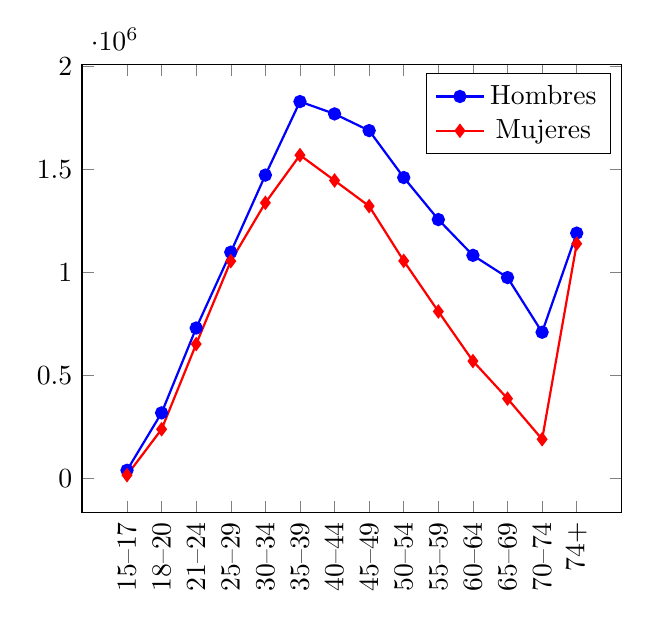
\begin{tikzpicture}
	\begin{axis}[legend style={anchor=north east},
	symbolic x coords={15--17,18--20,21--24,25--29,30--34,35--39,40--44,45--49,50--54,55--59,60--64,65--69,70--74,74+}, xtick=data, x tick label style={rotate=90,anchor=east}]
	\addlegendentry{Hombres}
	\addplot[mark=*,thick,blue] coordinates {
		(15--17,39341)
		(18--20,318037)
		(21--24,729846)
		(25--29,1097874)
		(30--34,1472038)
		(35--39,1828905)
		(40--44,1768957)
		(45--49,1688069)
		(50--54,1460193)
		(55--59,1256212)
		(60--64,1082591)
		(65--69,974768)
		(70--74,709285)
		(74+,1190514)
	};
	
	\addlegendentry{Mujeres}
	\addplot[mark=diamond*,thick,red] coordinates {
		(15--17,15697)
		(18--20,238534)
		(21--24,651961)
		(25--29,1054377)
		(30--34,1337432)
		(35--39,1568926)
		(40--44,1445740)
		(45--49,1321330)
		(50--54,1055472)
		(55--59,810168)
		(60--64,569461)
		(65--69,387158)
		(70--74,189829)
		(74+,1138945)
	};
	
	
	\end{axis}
	\end{tikzpicture}
	}
	\caption{Último censo de conductores según género segmentado por edades. Fuente: Dirección General de Tráfico (\url{dgt.es}).}
	\label{fig:drivers-census}
\end{marginfigure}
\subsection{Restricciones}

\begin{itemize}
	\item El sistema multiagente hará uso de \gls{dvu} como agentes, es decir, usando la tupla (conductor, vehículo) como un todo.
	\item La resolución máxima del modelo creado es de 1Hz.
	\item En el caso de los modelos que hacen uso de redes neuronales artificiales, no se pueden explicar las razones del comportamiento inferido.
\end{itemize}

\section{Estructura de la tesis}
\label{ch:intro:structure}

La tesis está estructurada de la siguiente manera:

En los capítulos \ref{ch:sota-traffic-simulators-and-mas}, \ref{ch:sota-ci} y \ref{ch:sota-behavior-models} se expone la revisión realizada del estado de la cuestión donde se explica en qué punto se encuentra la literatura de los temas en los que se apoya la presente tesis.

En el capítulo XXX se explica el método seguido para la confirmación de la hipótesis describiendo además las instrumentaciones, los conjuntos de datos obtenidos, las técnicas utilizadas y las aplicaciones desarrolladas.

Por último en el capítulo \ref{ch:conclusions} se exponen los resultados y las conclusiones extraídas de la tesis. Además, tras las conclusiones se indican una serie de posibles líneas futuras de trabajo consideradas interesantes tras la realización de la tesis.
